\documentclass[conference]{IEEEtran}
\documentclass{article}
\IEEEoverridecommandlockouts
% The preceding line is only needed to identify funding in the first footnote. If that is unneeded, please comment it out.
\usepackage{cite}
\usepackage{amsmath,amssymb,amsfonts}
\usepackage{graphicx}
\usepackage{textcomp}
\usepackage{xcolor}
\usepackage{titlesec}
\usepackage{textcomp}
\usepackage{epsfig}
\usepackage{algpseudocode}
\usepackage{pgfplots}
\usepackage{tikz}
\usepackage{hyperref}
\usepackage{graphicx}
\pgfplotsset{width=10cm,compat=1.9}
 \usepgfplotslibrary{external}



\usepackage[linesnumbered,ruled,vlined]{algorithm2e}
\def\BibTeX{{\rm B\kern-.05em{\sc i\kern-.025em b}\kern-.08em
    T\kern-.1667em\lower.7ex\hbox{E}\kern-.125emX}}

\usepackage[ruled,vlined]{algorithm2e}

\tikzexternalize 
\begin{document}

\title{FINDING WORDS IN ASCENDING OR DESCENDING ORDER \\
\textit{\Large{Indian Institute of Information technology, Allahabad }}\\
\text{\Large{DAA ASSIGNMENT-2 , GROUP 8}}
}
\author{\IEEEauthorblockN{Swaraj Bhosle}
\IEEEauthorblockA{ \text{IIT2019024}}
\and
\IEEEauthorblockN{Ritesh Raj}
\IEEEauthorblockA{ \text{IIT2019025}}
\and
\IEEEauthorblockN{Utkarsh Garg}
\IEEEauthorblockA{ \text{IIT2019026}}
}

\maketitle
{\textbf{\textit{Abstract: In this Paper we have devised an algorithm to find the number of valid English words which have ascending(A to Z) or descending(Z to A) ordered characters.
\\ }}}
\maketitle

\section{INTRODUCTION}\\
In computer science, the process of searching a 
string in a given set of strings is known as 
String Searching. We have created a text file 
containing at least $1000$ valid English words. 
Basically ascending characters in a string 
means all the characters should be in a 
alphabetical order i.e from A to Z and the 
descending order means all the characters 
should be in a reverse alphabetical order i.e 
from Z to A. For creating a new algorithm from 
scratch, we look into the many crucial aspects 
of algorithm designing and analysis.The 
algorithm created is tested for different sample 
test cases for time complexity, space 
complexity and accuracy. In our case 
\\ This report further contains - 
\begin{itemize}
    \item Algorithm Description.
    \item Algorithm And  Analysis.
    \item Time Complexity Analysis 
    \item Conclusion\
\end{itemize}

\section{ALGORITHM DESIGN}\\
We are using a file system in our algorithm as 
our input is stored in the file. Our algorithm 
will first of all read the input from the txt file. We have created the \textit{input.txt} file and all the input strings are inside this file.\\
\\\textbf{Step1 :}
First thing we will open the \textit{input.txt} file and will read the input for the programme. 
\\To read the information from a file into your 
programme we have to use the extraction 
operator $>>$  just as we use that operator to 
input information from the keyboard. The only 
difference is that we use an if stream or of stream object instead of the cin object. 
\\\\\textbf{Step2 :}
check whether the file is opened or 
not. i.e the open fails if the file doesn't exist, or if it can't be read. a failure can be detected with the code like !(logical not) operator 
\\\\\textbf{Step3 :}
create the character array of $MAX\_SIZE$ of $1000$. We will store the input string from the file into this character array
\\\\\textbf{Step4 :}
Traverse through each input string 
from .txt file.
\\\\\textbf{Step5 :}
create two different character arrays 
and store the input string in these two character 
arrays differently. 
\\\\\textbf{Step6 :}
Sort one of the above taken arrays in 
alphabetical order (A to Z) and sort the other 
array in reverse alphabetical order (Z to A)
\\\\\textbf{Step7 :}
compare the original string with these 
two created ascending and descending strings. 
If the original string matches one of the two 
strings then count it. 
\\\\\textbf{Step8 :}
print the count number.
\\\\\textbf{Step9 :}
close the opened file 
\\\\\textbf{\textit{Advantages of using merge sort:- }}
 It is quicker for larger lists because unlike 
insertion and bubble sort it doesn't go through the 
whole list several times. 
It has a consistent running time, carries out 
different bits with similar  times in a stage. 


\section{ALGORITHM AND ANALYSIS}\\
\begin{algorithm}[H] 
    \caption{Algorithm}
    \KwIn{string from the text 
document.}
    \KwOut {The number of English words that 
have ascending or descending characters}
    \DontPrintSemicolon
    \SetKwFunction{FMain}{Main}
    \SetKwProg{Fn}{Function}{:}{}
    \Fn{\FMain{}}{
           \\\textit{Declare an input file steam}
         \\\textbf{ifstream inFile}
          \\\textit{open the file stream}
        \\\textbf{inFile.open("input.txt")}; 
        
        \\\textit{Check that the file was opened }\\
         \If{$($ file can’t open $)$}{
                $Exit$\;
            }
        \\\textit{create the char array of MAX\_SIZE} 
          \\\textbf{char str[MAX\_SIZE]} 
        \\\textit{assign count equal to zero} 
         \\\textbf{ count = 0} 
         
         \While{\textit{inFile $>>$ str}}
         {
           \\\textit{Store the length of string in l }
             \\\textbf{ n = strlen(str) }
             \\\textit{create two char array of MAX_SIZE}
              \\\textbf{char asc[MAX\_SIZE]  }
               \\\textbf{char dsc[MAX\_SIZE]  }
            \\\textit{store str string in both asc and dsc array }
              
                 \For{$i \gets 0$ \textbf{ to } $n$}
                 {
                 $asc[i]$ = $str[i]$\\
                 $dsc[i]$ = $str[i]$
                }
            
        
         \\\textit{Sort asc array in ascending order }
        \\\textbf{merge\_sort(asc, asc + l) }
           \\ \textit{Sort the dsc array in descending order} 
        \\\textbf{merge\_sort(dsc,dsc+l,greater$<$char$>()$);} 
        \\\textit{compare the str string with dsc and asc array} 
        \\\textbf{if $(str==asc $ or $ str==dsc)$ }
          \\\textbf{count++; }
             \\\textit{if it matches any one of them then count it. }
             
    } 
       \\\textbf{print count }

 }
\end{algorithm}



   
\section{TIME CALCULATION }\\
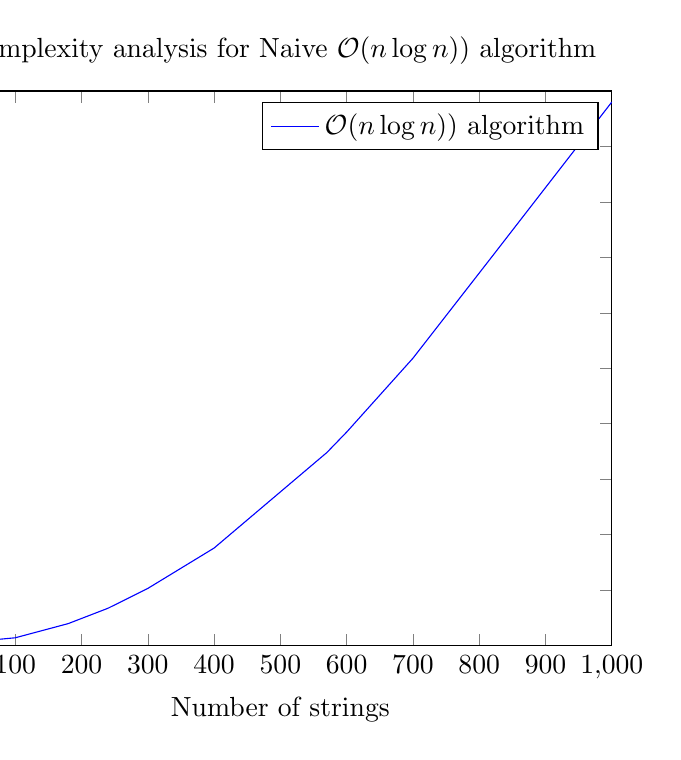
\begin{tikzpicture}[trim left=1cm]
\begin{axis}[
    title={Complexity analysis for Naive \begin{math} \mathcal{O}(n\log{}n)\end{math}) algorithm},
    xlabel={Number of strings},
    ylabel={Time(in ms) [t]},
     xmin=0, xmax=1000,
    ymin=0, ymax=100,
    xtick={100,200,300,400,500,600,700,800,900,1000},
    ytick={0,10,20,30,40,50,60,70,80,90,100}
]

\addplot[
    color=blue,
    mark=dot,
    ]
    coordinates {
    (0,0.3)(100,1.4)(180,3.96)(240,6.73)(300,10.3)(400,17.58)(570,34.79)(600,38.49)(700,51.81)(820,70.24)(1000,98)
    };
    \legend{\begin{math} \mathcal{O}(n\log{}n)\end{math}) algorithm}
   \end{axis}
   
\end{tikzpicture}




 \begin{tabular}{||c c||} 
 \hline
 No. of Words & Execution Time(ms) \\ [1.0ex] 
 \hline\hline
 100 & 1.4 \\ 
 \hline
 250 & 4 \\
 \hline
 500 & 34\\
 \hline
 800 & 70 \\
 \hline
 1000 & 98 \\
 \hline

\end{tabular}

\\\\
\section{TIME COMPLEXITY}\\
Let the average size of all strings be N.
Then we merge sort the string in ascending and 
descending order and compare the obtained strings 
with the original string, and if the string matches 
with any of the sorted strings then we increment the 
answer.\\ 
The time complexity will be \begin{math} \mathcal{O}(n\log{}n)\end{math}) due to the 
merge sort algorithm in a best, average and worst 
case.\\ 
The time complexity will be affected due to the 
merge sort in sorting the 1D array and the total 
time complexity will become \begin{math} \mathcal{O}(n\log{}n)\end{math}) in 
all the cases i.e. best case, worst case and 
average. 
\begin{math}
\end{math}
\\\\\\\\\textbf{Best Case : }

\begin{math}
\mathcal{O}(n) + \mathcal{O}(n\log{}n) + \mathcal{O} => \mathcal{O}(n\log{}n)
\end{math}
\\\textbf{Average Case : }


\begin{math}
\mathcal{O}(n) + \mathcal{O}(n\log{}n) + \mathcal{O} => \mathcal{O}(n\log{}n)
\end{math}
\\\textbf{Worst Case : }


\begin{math}
\mathcal{O}(n) + \mathcal{O}(n\log{}n) + \mathcal{O} => \mathcal{O}(n\log{}n)
\end{math}
\begin{center}
 \begin{tabular}{||c c c||} 
 \hline
  BEST & AVERAGE & WORST CASE  \\  
 \hline\hline
 \begin{math} \mathcal{O}(n\log{}n)
\end{math} & \begin{math} \mathcal{O}(n\log{}n)
\end{math} & \begin{math} \mathcal{O}(n\log{}n)
\end{math} \\ 
 \hline
\end{tabular}
\end{center}



\section{CONCLUSION}
Merge sort is one of the most efficient sorting 
algorithms. It works on the principle of Divide and 
Conquer. Merge sort repeatedly breaks down a list 
into several sub lists until each sub list consists of a single element and merging those sub lists in a manner that results into a sorted list in logarithmic time. 
\\This algorithm works as the string gets passed through the sorting algorithm and sorted in ascending and descending order which helps in 
comparing with the initial string of the text 
document and calculating the number of english 
words that are in ascending or descending 
characters. 

\section{REFERENCES}
\begin{enumerate}
    \item \url{  http://www.fredosaurus.com/notes-cpp/io/readtextfile.html }
    \item \url{ https://www.tutorialspoint.com/cplusplus/cpp_files_streams.html }
    \item \url{ https://www.geeksforgeeks.org/program-sort-string-descending-order}
\end{enumerate}
\end{document}